\chapter{Results}

The result of this project is a functional prototype of an interactive fluid
simulator. A game designer can use the modified version of Blender to add
fluids into a game built with the Blender Game Engine. Basic functionality in
the simulation and game logic have been achieved, laying the groundwork for
more complex physical phenomenon as well as more interesting interactions.


\section{Performance}
    
The performance of the project was benchmarked on two modern GPUs, an NVIDIA
GTX 480 and an AMD FirePro V7800. The GTX 480 has 480 CUDA Cores and 1.5GB of
video memory while the FirePro V7800 has 1440 Stream processors and 2GB of
video memory. The number of cores and processors do not directly correspond to
performance, as can be seen from the timings presented in Figure 7.1.


In addition to benchmarking the project, the CUDA SPH implementation from
Krog\cite{Krog2010} was run on with the GTX 480. As shown in Figure 7.1 RTPS is
not yet as efficient as SimpleSPH. Comparisons with CPU implementations were
not carried out as the literature has shown the wide gap in performance makes
the CPU non-competitive.\cite{Hoetzlein}\cite{Krog2010}


\begin{figure}[!htc]
 		\centering
		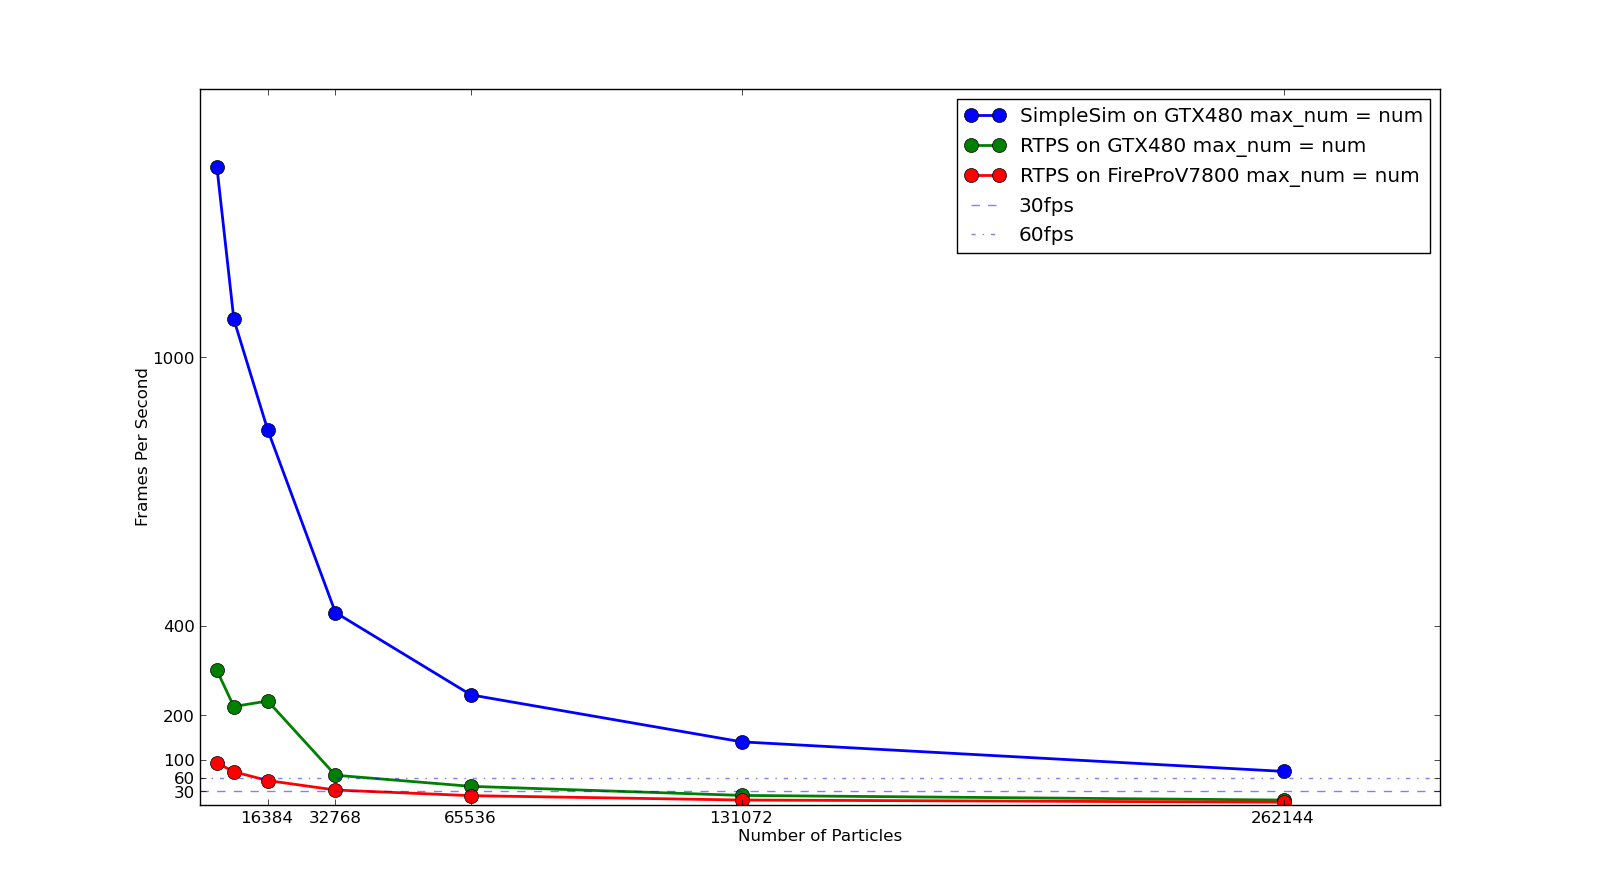
\includegraphics[scale=0.5]{figures/maxnum_eq_num_fps.png}
		\label{fig:logic}
        \caption{ SPH Timings }
\end{figure}

For these timings the only parameter varied is the maximum number of particles.
For each case the maximum number of particles is emitted and the timing of each
function call is averaged over 1000 iterations. Figures 7.1 and 7.2 are
measured in Frames Per Second for which a higher number is more desirable.
Figures 7.3 through 7.5 are given in milliseconds in which case a lower number
is better.

\pagebreak

One logical use scenario would involve setting a large maximum number of
particles and only using a relatively small subset of them. This will make the
radius of each particle smaller if the domain size remains fixed, allowing the
user to get a more detailed simulation. It turns out that this use case is much
more efficient than setting the maximum number of particles to the amount to be
used as can be seen in Figure 7.2. 

\begin{figure}[!htc]
 		\centering
		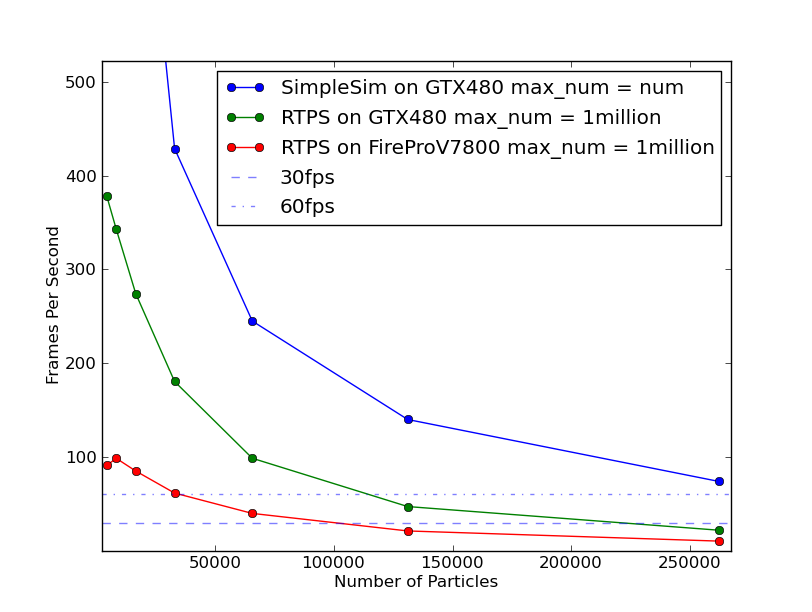
\includegraphics[scale=0.5]{figures/maxnum_eq_1mill_fps.png}
		\label{fig:logic}
        \caption{ SPH Timings with maximum number of particles set to 1 million }
\end{figure}

\pagebreak

One can see from Figure 7.3 that the Density and Force calculations are by far
the most expensive routines. These routines have the most memory accesses, and
the more neighbors that each particle must calculate the more memory accesses
these routines use. 

\begin{figure}[!htc]
 		\centering
		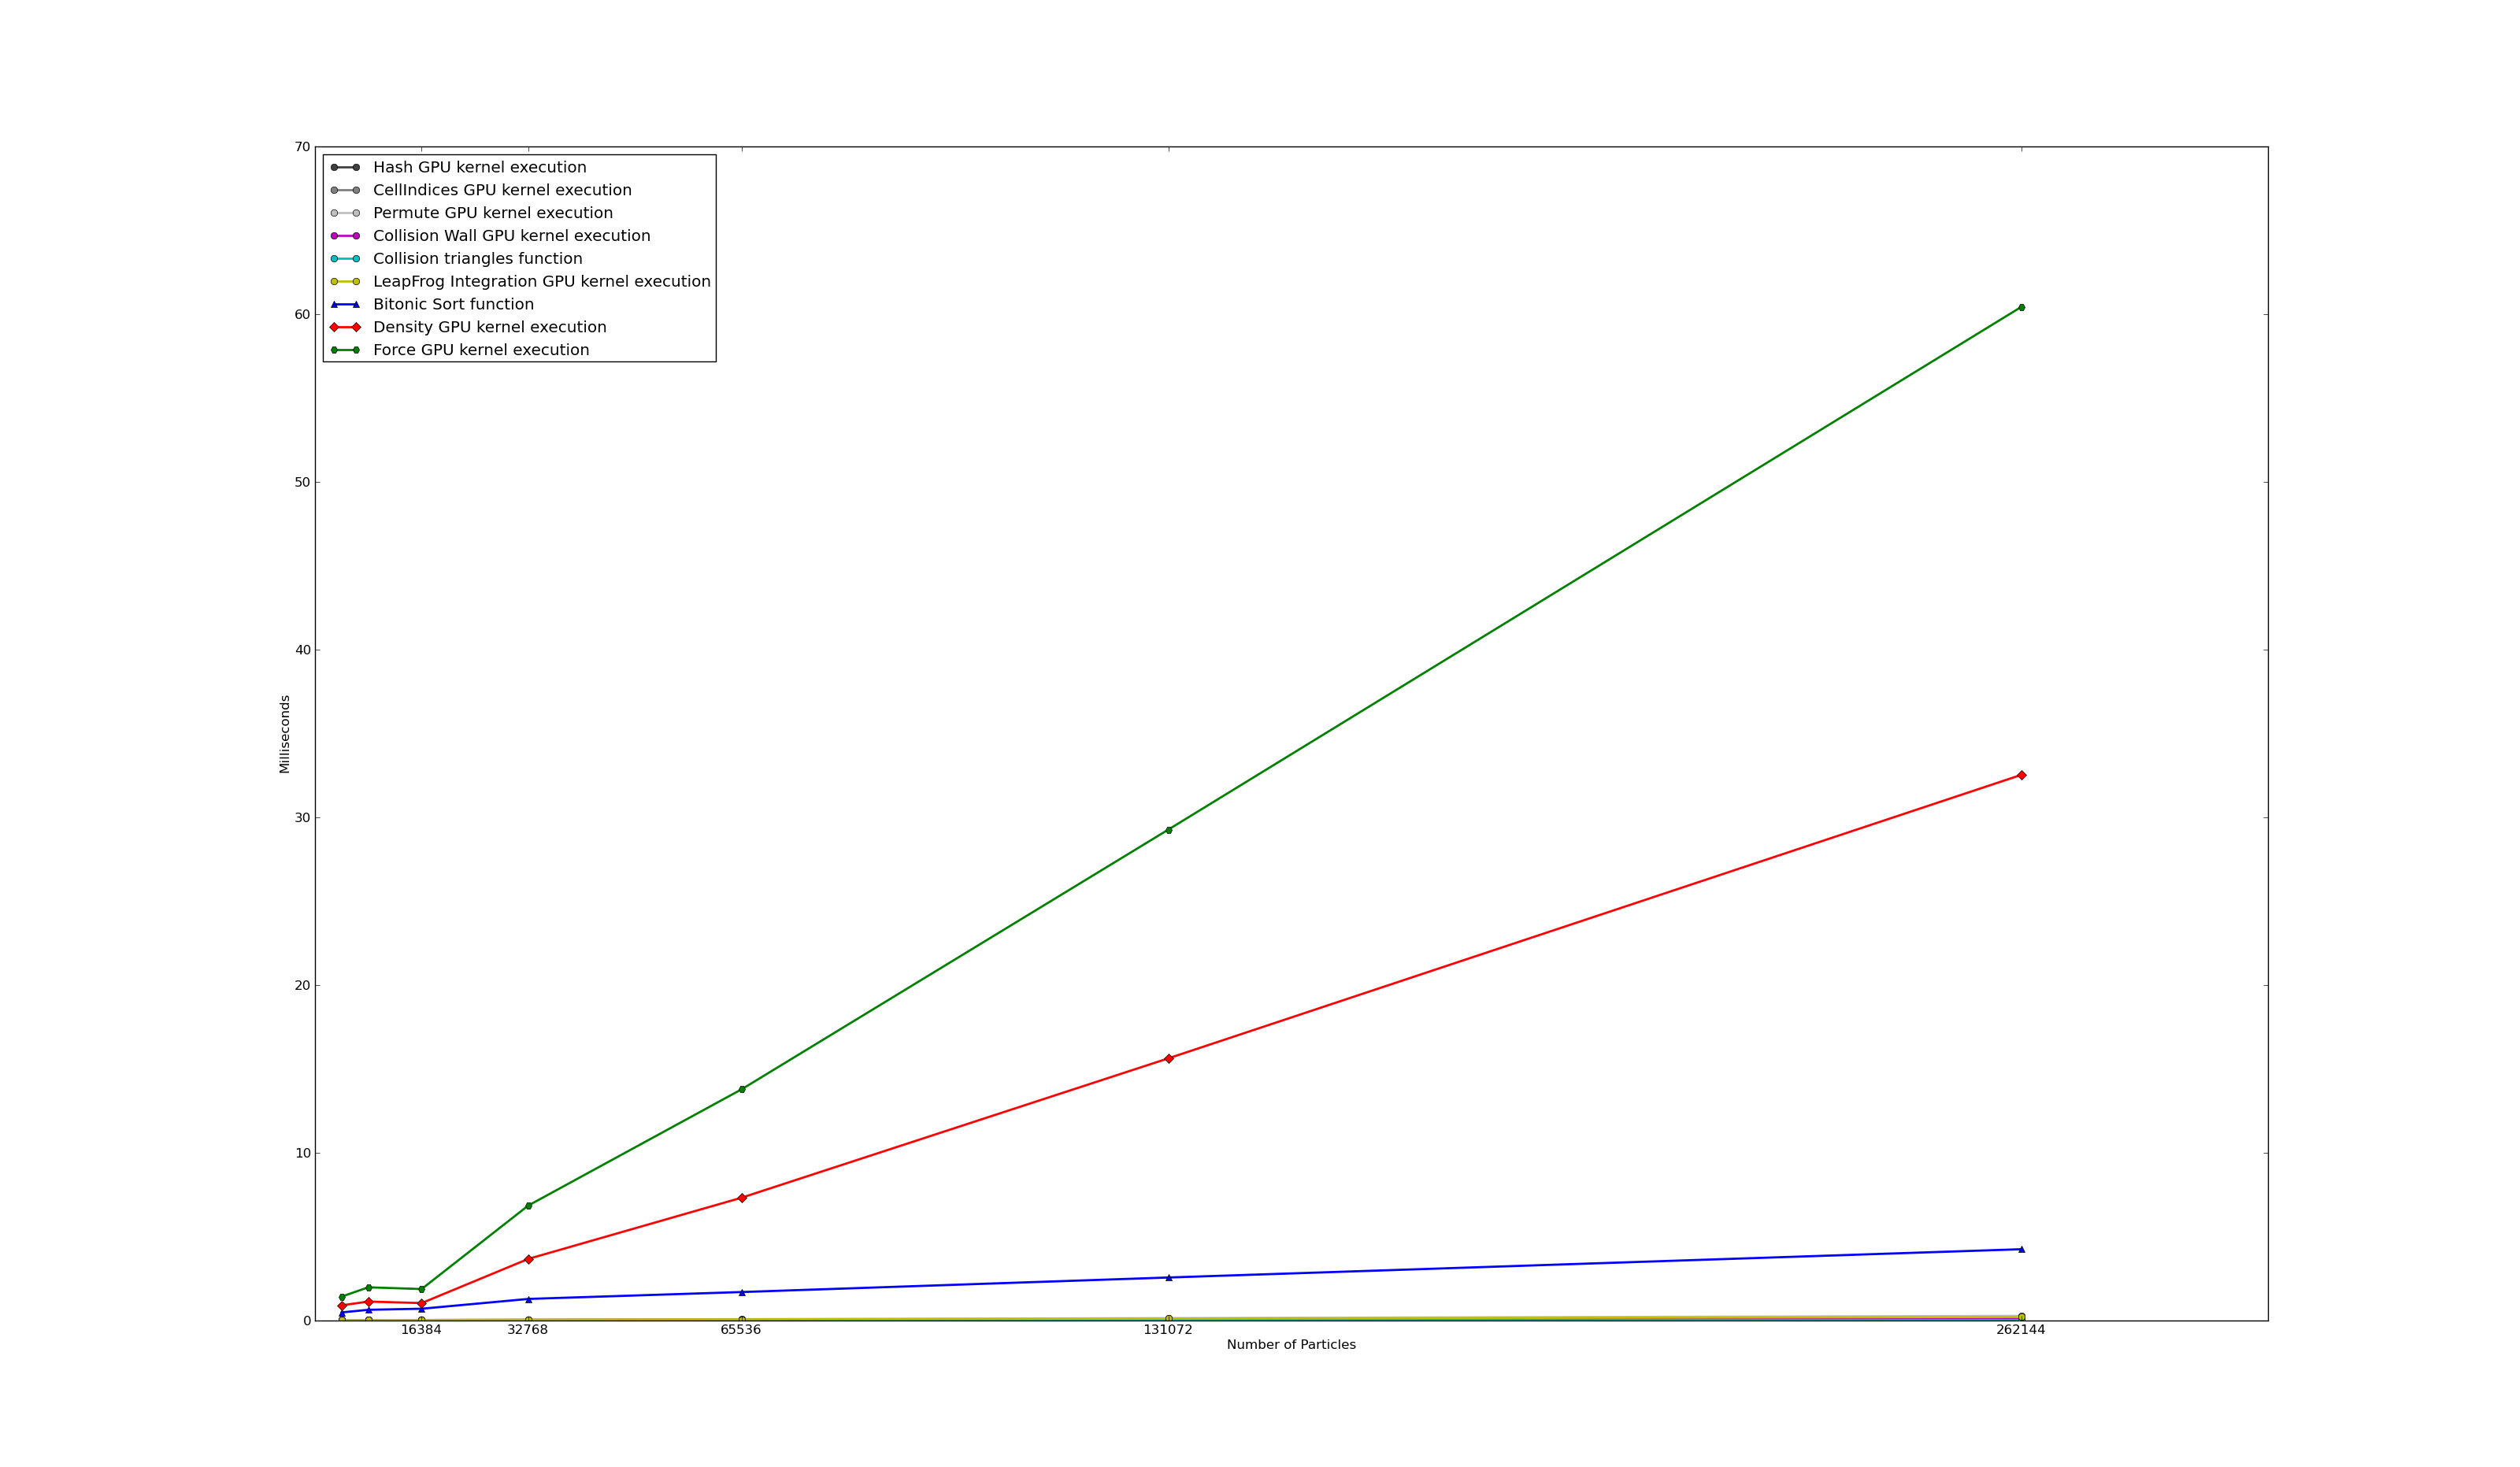
\includegraphics[scale=0.4]{figures/nv_kernel_num.png}
		\label{fig:logic}
        \caption{ GPU timings for each kernel }
\end{figure}


\pagebreak

Figure 7.4 shows that the density and force kernels increase in computational
time much quicker when the number of particles is equal to the maximum number.
This is most likeley due to a higher saturation of neighboring particles when
the number of particles approaches the maximum number, thus leading to more memory accesses.

\begin{figure}[!htc]
 		\centering
		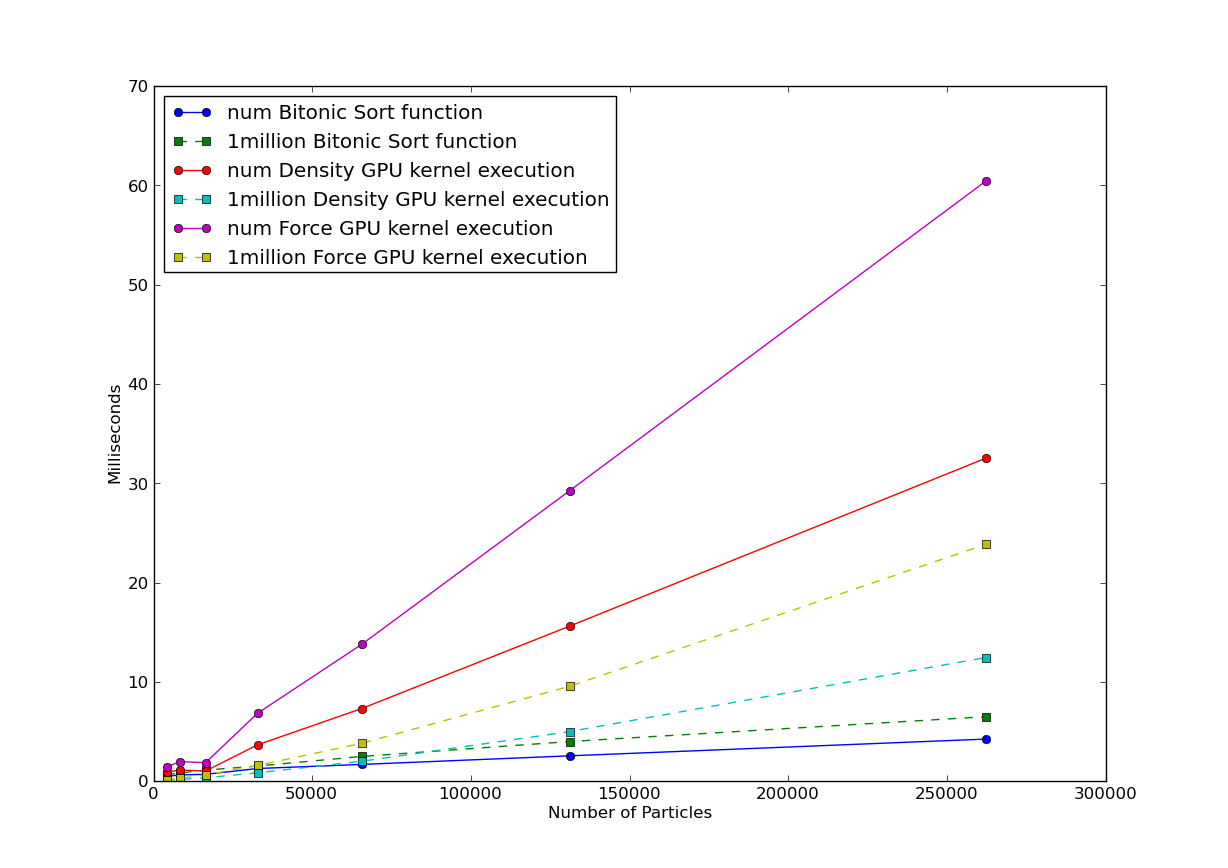
\includegraphics[scale=0.5]{figures/nv_kernel_neighbor.png}
		\label{fig:logic}
        \caption{ Comparison of max number = 1 million with max number = number of particles }
\end{figure}

\pagebreak
Figure 7.5 shows the timings for the most expensive kernels on each video card,
suggesting that the ATI card is slower by a constant factor.

\begin{figure}[!htc]
 		\centering
		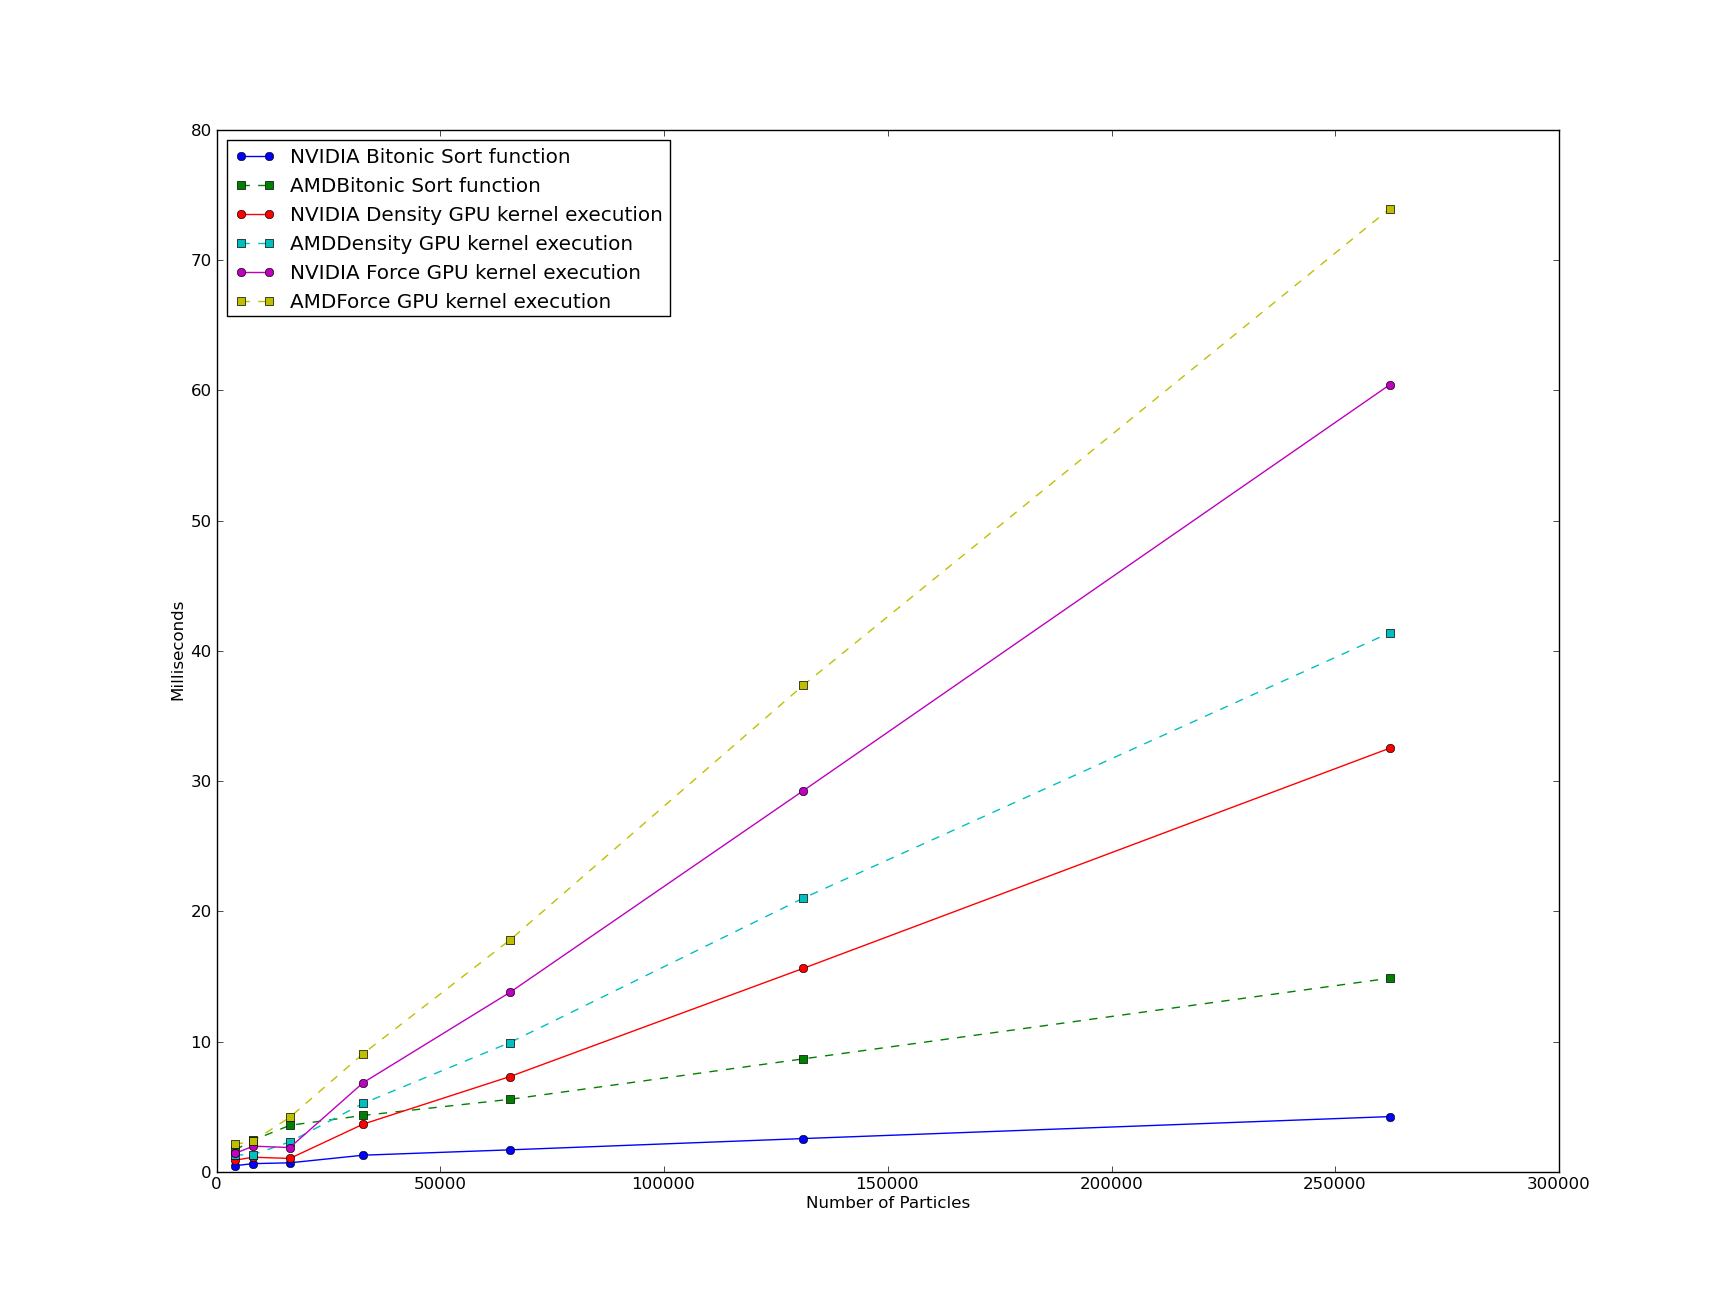
\includegraphics[scale=0.4]{figures/nv_vs_ati.png}
		\label{fig:logic}
        \caption{ GPU timings for the most expensive kernels on each card }
\end{figure}


\pagebreak
\section{Community}


An important aspect of this project is adoption by the game design community.
Acceptance by the Blender community entails benefits such as user generated
tutorials and developer support. The project has enjoyed a preliminary amount
of success in this regard, being featured on the primary news source for
the Blender community.\footnote{
\url{http://www.blendernation.com/2011/01/03/fluids-in-real-time-with-opencl/}
\\ 
\url{
http://www.blendernation.com/2011/04/20/ian-johnson-fluid-simulation-blender-game-engine-using-opencl/
} }

Builds were compiled for the Windows, Mac and Linux operating systems and
distributed to members of the community for testing. These members have already
provided valuable feedback, crash reports and even demos.\footnote{ \url{http://www.youtube.com/watch?v=s2QBRazykEA}} 

\begin{figure}[!htc]
 		\centering
		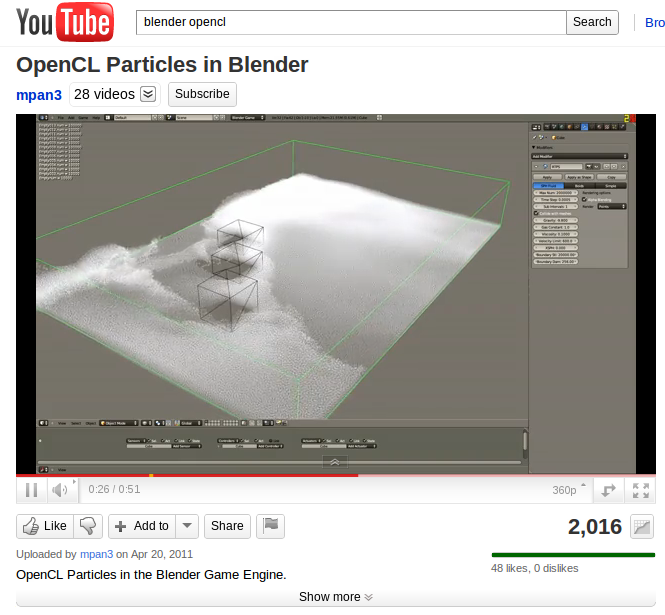
\includegraphics[scale=0.5]{figures/youtube.png}
		\label{fig:logic}
        \caption{ Artist demo }
\end{figure}

The project has also recieved support from developers with regards to
integrating the RTPS library with Blender. As the code improves and the
integration becomes tighter it is expected that more developers will be willing
and able to help.


